\documentclass{article}
\usepackage[paper=a4paper,margin=0.5in]{geometry}
\usepackage{hyperref}
\usepackage{gensymb}
\usepackage{graphicx}
\begin{document}
	\null\hfill\begin{tabular}[t]{l@{}}
	\textit{CSCI 580 Unofficial Final Study Guide}\\
	\end{tabular} \\ \\
\section{Markov Decision Processes and Bellman Equations}
Review 4x3 Grid World\\
MDPs consist of 
\begin{itemize}
	\item A set of States $s\in S$
	\item A set of Actions $a\in A$
	\item A Transition Function $T(s,a,s')$
	\item A Reward Function $R(s,a,s')$
	\item A start state (optional)
	\item A terminal state (optional)
\end{itemize}
Markov decision processes attempt to find the optimal policy $\pi*(s)$ which is the best decision at any given state $(s)$ at any particular iteration $k$.\\
We can do this by starting with a vector of all states initialized to 0, called $V_0$. Next utilize $V_{k-1}$ to calculate $V_k$ with the \textbf{Bellman Equation}:
$$max\Sigma T(s,a,s')(R(s,a,s')+\gamma V_{k-1}(s'))$$
Where $\gamma$ is the discount (given). Remember, even though Dr. J says that this exponentially increases as $k$ increases, this increase is built in. Just multiple $V_{k-1}(s')$ by $\gamma$
\subsection{Policy Evaluation}
The MDP where we attempt to create the best action $\pi*$ for any state $s$
\subsection{Policy Extraction}
Perform a one step expecti-max to calculate
$$argmax\Sigma T(s,a,s')(R(s,a,s')+\gamma V_{k-1}(s'))$$
\section{Intro to Machine Learning}
\subsection{1R}
Attempts to characterize and predict a model based off of a single attribute. 1R is not capable of evaluating numerical data. \\
Remember the weather.nominal.arff, specifically looking at Outlook. For 14 datasets, we can analyze each class within Outlook: Sunny, Overcast, Rainy.
\begin{itemize}
	\item Sunny, 2 Yes, 3 no. The majority of this group is no's with an error of 2/5
	\item Overcast, 4 Yes, 0 no. The entirety of this group is yes with an error of 0/4.
	\item Rainy, 3 yes, 2 no. The majority of this group is yes with an error of 2/5.
\end{itemize}
So for Outlook, we have an error of 4/14. We repeat this process for all other attributes within the dataset, and choose the attribute with the smallest error. For arguments sake, we'll assume Outlook is the smallest error. Thusly, we'll choose the prediction of instances based off of their Outlook status. If a instance is Sunny, we will say don't play. If an instance is Overcast, we'll say yes play. If an instance is Rainy, we'll say yes play.
\subsection{Na\"ive Bayes}
In contrast to 1R, \textbf{Na\"ive Bayes} takes into consideration all attribute within an instance.\\
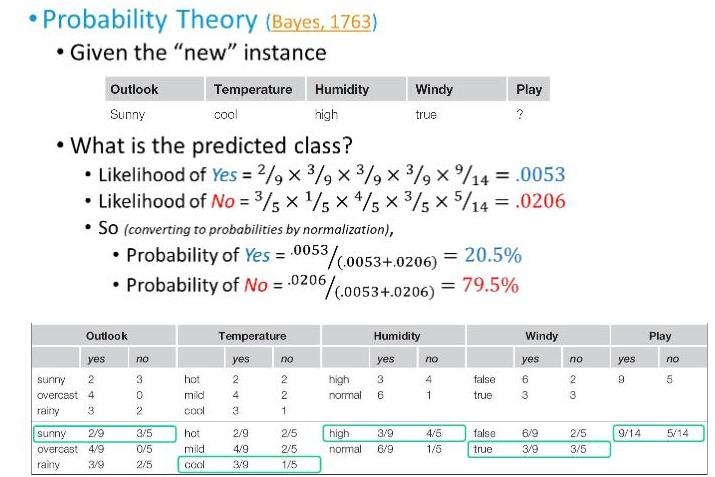
\includegraphics[scale=0.5]{pics/naivebayes.png}
\section{Decision Trees}
\subsection{Iterative Dichotomizer 3 (ID3)}
For any attribute within the dataset, calculate the \textbf{information gain}. To calculate information gain, we must first calculate the entropy of each class within the attribute, then the entropy of the class as a whole.\\
This one is incredibly intense to write out. Look at your homework for calculating entropy
\end{document}
